\title{Лекция 12\\Представление в базе знаний предметных областей}
\author[]{Шункевич Д.В.}
\institute[]{Белорусский государственный университет информатики и радиоэлектроники}

\begin{frame}
	\titlepage
\end{frame}

\begin{frame}{\\Содержание лекции}
	\topline
	\justifying
	Понятие знания, типология знаний. Понятие предметной области, структурная спецификация предметной области, роли понятий в рамках предметной области. Понятие частной предметной области, родственной предметной области, виды частных предметных областей. Различные виды иерархии предметных областей, пересечения предметных областей.
\end{frame}

\begin{frame}{\\Знание}
	\topline
	\justifying
	\begin{SCn}
		\scnheader{знание}
		\scnidtf{синтаксически корректная (для соответствующего языка) и семантически целостная информационная конструкция}
		\scnsubset{информационная конструкция}		
		\scnrelfrom{покрытие}{
			вид знаний\\
			\scnidtf{множество \underline{всевозможных} видов знаний}			
			\scntext{примечание}{Тот факт, что семейство \textit{видов знаний} является \textit{покрытием} Множества всевозможных \textit{знаний}, означает то, что каждое \textit{знание} принадлежит по крайней мере одному выделенному нами \textit{виду знаний}}						
		}		
	\end{SCn}
\end{frame}

\begin{frame}{\\Вид знаний}
	\topline
	\justifying
	\vspace{5mm}
	\footnotesize{
		\begin{SCn}
			\scnheader{вид знаний}
			\scnhaselement{спецификация}		
			\begin{scnindent}
				\scnidtf{описание заданной сущности}
				\scnsuperset{спецификация материальной сущности}
				\scnsuperset{спецификация обратной сущности, не являющейся множеством}			
				\scnsuperset{спецификация множества}
				\scnsuperset{семантическая окрестность}
				\scnsuperset{однозначная спецификация}
				\scnsuperset{сравнительный анализ}
				\scnsuperset{достоинства}
				\scnsuperset{недостатки}
				\scnsuperset{структура специфицируемой сущности}
				\scnsuperset{принципы, лежащие в основе}
				\scnsuperset{обоснование предлагаемого решения}
			\end{scnindent}
			\scnhaselement{сравнение}		
			\scnhaselement{высказывание}
			\scnhaselement{формальная теория}		
			\scnhaselement{предметная область}
		\end{SCn}
	}
\end{frame}

\begin{frame}{\\Вид знаний}
	\topline
	\justifying
	\begin{SCn}
		\scnheader{вид знаний}
		\scnhaselement{предметная область и онтология}
		\scnhaselement{метазнание}
		\scnhaselement{задача}
		\scnhaselement{план}		
		\scnhaselement{протокол}		
		\scnhaselement{результативная часть протокола}		
		\scnhaselement{метод}		
		\scnhaselement{технология}
	\end{SCn}
\end{frame}

\begin{frame}{\\Типология знаний}
	\topline
	\justifying
	\vspace{5mm}
	\footnotesize{
		\begin{SCn}
			\scnheader{знание}
			\begin{scnrelfromset}{разбиение}
				\scnitem{декларативное знание}
					\begin{scnindent}
						\scnidtf{\textit{знание}, имеющее \underline{только} \textit{денотационную семантику}, которая представляется в виде семантической \textit{спецификации} системы \textit{понятий}, используемых в этом \textit{знании}}
					\end{scnindent}
				\scnitem{процедурное знание}
					\begin{scnindent}
						\scnidtf{\textit{знание}, имеющее не только \textit{денотационную семантику}, но и \textit{операционную семантику}, которая представляется в виде семейства \textit{спецификаций агентов}, осуществляющих интерпретацию \textit{процедурного знания}, направленную на решение некоторой инициированной \textit{задачи}}
						\scnidtf{функционально интерпретируемое знание, обеспечивающее решение либо конкретной задачи, либо некоторого множества инициируемых задач}
						\scnsuperset{задача}
						\scnsuperset{план}
						\scnsuperset{метод}
						\scnsuperset{навык}
					\end{scnindent}				
				
			\end{scnrelfromset}
		\end{SCn}
	}
\end{frame}

\begin{frame}{\\Типология знаний}
	\topline
	\justifying
	\footnotesize{
		\begin{SCn}
			\scnheader{задача}
			\scnidtf{формулировка конкретной задачи}
			\scnsuperset{декларативная формулировка задачи}
			\scnsuperset{процедурная формулировка задачи}
			\scnheader{план}
			\scnidtf{план решения конкретной задачи}
			\scnidtf{контекст конкретной задачи, предоставляющий всю информацию для решения всех подзадач для указанной конкретной задачи}
			\scnidtf{описание системы подзадач некоторой задачи}
			\scnheader{метод}
			\scnidtf{обобщенное описание плана решения любой задачи из некоторого заданного класса задач}
			\scnheader{навык}
			\scnidtf{метод, детализированный до уровня элементарных подзадач}
		\end{SCn}
	}
\end{frame}

\begin{frame}{\\Предметная область}
	\topline
	\justifying
	\begin{SCn}
		\scnheader{предметная область}
		\scnidtf{sc-модель предметной области}
		\scnidtf{sc-текст предметной области}
		\scnidtf{sc-граф предметной области}
		\scnidtf{представление предметной области в \textit{SC-коде}}
		\scnsubset{знание}
		\scnsubset{бесконечное множество}
		\scntext{пояснение}{\textbf{\textit{предметная область}} -- это результат интеграции (объединения) частичных семантических окрестностей, описывающих все исследуемые сущности заданного класса и имеющих одинаковый (общий) предмет исследования (то есть один и тот же набор отношений, которым должны принадлежать связки, входящие в состав интегрируемых семантических окрестностей).}
	\end{SCn}
\end{frame}

\begin{frame}{\\Предметная область}
	\topline
	\justifying
	\\
	\footnotesize{
		\textbf{\textit{предметная область}} -- \textit{структура}, в состав которой входят:
		\begin{textitemize}
			\item{\textnormal{основные исследуемые (описываемые) объекты -- первичные и вторичные;}}
			\item{\textnormal{различные классы исследуемых объектов;}}
			\item{\textnormal{различные связки, компонентами которых являются исследуемые объекты (как первичные, так и вторичные), а также, возможно, другие такие связки -- то есть связки (как и объекты исследования) могут иметь различный структурный уровень;}}
			\item{\textnormal{различные классы указанных выше связок (то есть отношения);}}
			\item{\textnormal{различные классы объектов, не являющихся ни объектами исследования, ни указанными выше связками, но являющихся компонентами этих связок.}}
		\end{textitemize}
		При этом все классы, объявленные исследуемыми понятиями, должны быть полностью представлены в рамках данной предметной области вместе со своими элементами, элементами элементов и т.д. вплоть до терминальных элементов.
	}
\end{frame}

\begin{frame}{\\Роль элемента предметной области}
	\topline
	\justifying
	\begin{SCn}
		\scnheader{роль элемента предметной области}
		\scnidtf{ролевое отношения, связывающее предметные области с их ключевыми знаками}
		\scnidtf{роль ключевого элемента (знака ключевой сущностей) предметной области}
		\scnidtf{роль ключевого знака предметной области}
		\scnhaselement{класс объектов исследования\scnrolesign}
		\scnhaselement{максимальный класс объектов исследования\scnrolesign}
		\scnhaselement{ключевой объект исследования\scnrolesign}
		\scnhaselement{понятие, используемое в предметной области\scnrolesign}
		\scnhaselement{первичный исследуемый элемент предметной области\scnrolesign}
		\scnhaselement{вторичный исследуемый элемент предметной области\scnrolesign}
		\scnhaselement{неисследуемый элемент предметной области\scnrolesign}
	\end{SCn}
\end{frame}

\begin{frame}{\\Класс объекта исследования}
	\topline
	\justifying
	\footnotesize{
		\begin{SCn}
			\scnheader{класс объектов исследования\scnrolesign}
			\scnidtf{быть классом \underline{первичных} (для данной предметной области) объектов исследования\scnrolesign}
			\scntext{примечание}{Понятие \underline{первичного} объекта исследования для предметной области является понятием \underline{относительным} и абсолютно не зависит от типа и уровня сложности этого объекта.
				
			Особого внимания требуют те \textit{классы объектов исследования}, которые носят наиболее общий характер  которым соответствуют \textit{предметные области и онтологии} \underline{высокого уровня}. Здесь важна продуманная система декомпозиции всего множества окружающих нас сущностей на иерархическую систему \textit{классов объектов исследования}, которой соответствует иерархическая система \textit{предметных областей и онтологий}, определяющая направления \underline{наследования свойств} исследуемых объектов.}
			\scnrelfrom{второй домен}{класс}
		\end{SCn}
	}
\end{frame}

\begin{frame}{\\Класс объекта исследования}
	\topline
	\justifying
	\begin{SCn}
		\scnheader{максимальный класс объектов исследования\scnrolesign}
		\scnidtf{класс объектов исследования, для которого \underline{в заданной} (!) предметной области отсутствует другой класс объектов исследования, который был бы его надмножеством\scnrolesign}
		\scntext{примечание}{В некоторых предметных областях может быть \underline{несколько} максимальных классов объектов исследования}
		\scnheader{ключевой объект исследования\scnrolesign}
		\scnidtf{особый объект исследования\scnrolesign}
		\scnidtf{быть знаком особого исследуемого объекта в рамках заданной предметной области\scnrolesign}
		\scnidtf{объект исследования, обладающий особыми свойствами\scnrolesign}
	\end{SCn}
\end{frame}

\begin{frame}{\\Ключевой элемент предметной области}
	\topline
	\justifying
	\begin{SCn}
		\scnheader{ключевой элемент предметной области\scnrolesign}
		\scnidtf{входящий в состав предметной области знак ключевой сущности\scnrolesign}
		\begin{scnrelfromset}{разбиение}
			\scnitem{понятие, используемое в предметной области\scnrolesign}			
			\scnitem{ключевой объект исследования\scnrolesign}						
		\end{scnrelfromset}
	\end{SCn}
\end{frame}

\begin{frame}{\\ Понятие, используемое в ПрО}
	\topline
	\justifying
	\begin{SCn}
		\scnheader{понятие, используемое в предметной области\scnrolesign}
		\scnidtf{понятие, используемое в заданной предметной области не в качестве одного из объектов исследования, а в качестве \underline{ключевого} понятия\scnrolesign}
		\scnsubset{используемое понятие\scnrolesign}
		\scnrelfrom{разбиение}{семантический тип используемого понятия}
		\begin{scnindent}
			\begin{scneqtoset}
				\scnitem{класс объектов исследования\scnrolesign}
				\scnitem{отношение, используемое в предметной области\scnrolesign}
				\scnitem{класс структур, используемый в предметной области\scnrolesign}
			\end{scneqtoset}
		\end{scnindent}		
	\end{SCn}
\end{frame}

\begin{frame}{\\ Понятие, используемое в ПрО}
	\topline
	\justifying
	\begin{SCn}
		\scnheader{понятие, используемое в предметной области\scnrolesign}		
		\scnrelfrom{разбиение}{полнота вхождения элементов понятия в данную предметную область}
		\begin{scnindent}
			\begin{scneqtoset}
				\scnitem{используемое понятие, все элементы которого входят в данную предметную область\scnrolesign}
				\scnitem{используемое понятие, не все элементы которого входят в данную предметную область\scnrolesign}				
			\end{scneqtoset}
		\end{scnindent}
		\scnrelfrom{разбиение}{наличие первого упоминания понятия}
		\begin{scnindent}
			\begin{scneqtoset}
				\scnitem{понятие, вводимое в данной предметной области\scnrolesign}
				\scnitem{понятие, которое в данной предметной области используется, но не вводится\scnrolesign}				
			\end{scneqtoset}
		\end{scnindent}			
	\end{SCn}
\end{frame}

\begin{frame}{\\ Понятие, используемое в ПрО}
	\topline
	\justifying
	\vspace{5mm}
	\begin{SCn}
		\scnheader{понятие, используемое в предметной области\scnrolesign}		
		\scnrelfrom{разбиение}{наличие определения понятия или объявления его неопределяемости с подробным пояснением и примерами}
		\begin{scnindent}
			\begin{scneqtoset}
				\scnitem{понятие, которое в данной предметной области определено или объявлено как неопределяемое\scnrolesign}
				\scnitem{понятие, которое в данной предметной области не имеет ни определения, ни указания факта его неопределяемости\scnrolesign}				
			\end{scneqtoset}
		\end{scnindent}
		\scnrelfrom{разбиение}{наличие исследования понятия}
		\begin{scnindent}
			\begin{scneqtoset}
				\scnitem{понятие, исследуемое в данной предметной области\scnrolesign}
				\scnitem{понятие, которое в данной предметной области используется, но не исследуется\scnrolesign}				
			\end{scneqtoset}
		\end{scnindent}			
	\end{SCn}
\end{frame}

\begin{frame}{\\Порядок исследования элементов ПрО}
	\topline
	\justifying
	\begin{SCn}
		\scnheader{первичный исследуемый элемент предметной области\scnrolesign}
		\scnidtf{знак первичного объекта исследования в рамках заданной предметной области\scnrolesign}		
		\scnheader{вторичный исследуемый элемент предметной области\scnrolesign}
		\scnidtf{знак вторичного объекта исследования в рамках предметной области\scnrolesign}
		\scnsuperset{связка элементов предметной области\scnrolesign}
		\scnsuperset{класс элементов предметной области\scnrolesign}
		\scnsuperset{структура элементов предметной области\scnrolesign}
	\end{SCn}
\end{frame}

\begin{frame}{\\Неисследуемый элемент ПрО}
	\topline
	\justifying
	\footnotesize{
		\begin{SCn}
			\scnheader{неисследуемый элемент предметной области\scnrolesign}
			\scnidtf{вспомогательный элемент предметной области, исследуемый в другой (смежной) предметной области\scnrolesign}
			\scntext{примечание}{С помощью неисследуемых элементов предметной области описываются и исследуются различные вида связи между элементами, исследуемыми в данной \textit{предметной области} с элементами, исследуемыми в других \textit{предметных областях}. 
				
			При этом \textit{связки}, компонентами которых являются как исследуемые, так и неисследуемые элементы данной \textit{предметной области} считаются \underline{исследуемыми} связками этой \textit{предметной области}. 
			
			Примерами неисследуемых элементов, напримр, геометрической \textit{предметной области} являются \textit{числа}, являющиеся \textit{значениями величин} таких \textit{параметров}, как \textit{расстояние}\scnsupergroupsign, \textit{длина}\scnsupergroupsign, \textit{площадь}\scnsupergroupsign, \textit{объем}\scnsupergroupsign, а также различные числовые \textit{отношения} (\textit{сложение}*, \textit{умножение}*, \textit{возведение в степень}*), теоретико-множественные \textit{отношения} (\textit{включение}*, \textit{объединение}*, \textit{пересечение}*, \textit{принадлежность}*)}
		\end{SCn}
	}
\end{frame}

\begin{frame}{\\Понятие}
	\topline
	\justifying
	\small{
		\begin{SCn}
			\scnheader{понятие}
			\scnidtf{концепт}
			\scnidtf{класс сущностей, который входит в состав по крайней мере одной предметной области в качестве (в роли) ключевого исследуемого понятия}
			\scntext{примечание}{Семейство всех введенных понятий -- это, своего рода, семантическая система координат, позволяющая специфицировать всевозможные сущности в смысловом пространстве.}		
			\scnidtf{класс сущностей, который по крайней мере в одной \textit{предметной области} "объявлен"{} как \textit{понятие} (вводимое, исследуемое или вспомогательное)}
			\scntext{примечание}{Каждому \textit{понятию} соответствует по крайней мере одна \textit{предметная область}, в которой это понятие является \textit{исследуемым понятием} и в которой рассматриваются основные характеристики этого \textit{понятия}. Если же в какой-либо \textit{предметной области} необходимо рассмотреть дополнительные связи этого \textit{понятия} с другими \textit{понятиями}, то оно объявляется как \textit{вспомогательное понятия}\scnrolesign.}			
		\end{SCn}
	}
\end{frame}

\begin{frame}{\\Понятие}
	\topline
	\justifying
	\begin{SCn}
		\scnheader{понятие}			
		\scnidtf{второй домен Отношения \textit{используемое понятие}*}
		\scnrelto{второй домен}{используемое понятие*}
		\scnidtf{класс сущностей (класс связок (в т.ч. отношение), класс классов (в т.ч. параметр), класс структур), который по крайней мере в одной \textit{предметной области} является \textit{используемым понятием}\scnrolesign}
	\end{SCn}
\end{frame}

\begin{frame}{\\Отношения, заданные на мн-ве ПрО}
	\topline
	\justifying
	\begin{SCn}
		\scnheader{отношение, заданное на множестве предметных областей}
		\scnhaselement{\scnkeyword{дочерняя предметная область*}}
		\scnhaselement{\scnkeyword{интеграция предметных областей*}}
		\scnhaselement{\scnkeyword{изоморфность предметных областей*}}
		\scnhaselement{\scnkeyword{гомоморфность предметных областей*}}
	\end{SCn}
\end{frame}

\begin{frame}{\\Дочерняя ПрО}
	\topline
	\justifying
	\vspace{5mm}
	\begin{SCn}
		\scnheader{дочерняя предметная область*}
		\scnidtf{частная предметная область*}
		\scnidtf{быть частной предметной областью*}
		\scnidtf{близлежащий потомок предметной области*}
		\scnidtf{сужение предметной области по классу объектов исследования*}
		\scnidtf{предметная область, детализирующая описание одного из классов объектов исследования другой (более общей) предметной области*}
		\scnidtf{предметная область, объединение классов объектов исследования которой является подмножеством объединения классов объектов исследования заданной предметной области*}
		\scniselement{бинарное отношение}
		\scniselement{ориентированное отношение}
		\scniselement{неролевое отношение}
		\scnsuperset{частная предметная область по классу первичных элементов*}
		\scnsuperset{частная предметная область по исследуемым отношениям*}
	\end{SCn}
\end{frame}

\begin{frame}{\\Дочерняя ПрО}
	\topline
	\justifying
	\begin{SCn}
		\scnheader{дочерняя предметная область*}
		\scntext{пояснение}{\textit{дочерняя предметная область*} -- бинарное ориентированное отношение, с помощью которого задается иерархия предметных областей путем перехода от менее детального к более детальному рассмотрению соответствующих исследуемых понятий.}
		\scntext{примечание}{Для любой \textit{предметной области} все свойства ее \textit{объектов исследования} \underline{наследуются} всеми ее \textit{дочерними предметными областями*}.}
	\end{SCn}
\end{frame}

\begin{frame}{}
	\topline
	\justifying
	\small{
		\begin{SCn}
			\scnheader{расширение семейства исследуемых отношений*}
			\scntext{пояснение}{Переход от одной предметной области к предметной области с тем же максимальным классом объектов исследования, но с расширенным семейством отношений и, возможно, с расширенным семейством явно выделенных классов объектов исследования (подклассов максимального класса).}
			\scnheader{переход к рассмотрению внутренней структуры объектов исследования*}
			\scntext{пояснение}{Переход от рассмотрения внешних связей объектов исследования к рассмотрению их "внутренней"{} структуры путем декомпозиции исследуемых объектов на части и путем включения в число исследуемых объектов тех, которые являются указанными частями.}			
		\end{SCn}
	}
\end{frame}

\begin{frame}{}
	\topline
	\justifying		
	\begin{SCn}		
		\scnheader{переход к рассмотрению структур из объектов исследования*}
		\scntext{пояснение}{Переход от описания заданного класса исследуемых объектов к описанию класса всевозможных множеств, элементами которых являются указанные объекты (например, переход от предметной области геометрических точек к предметной области геометрических фигур).}
	\end{SCn}
\end{frame}

\begin{frame}{\\Пример иерархии ПрО}
	\topline
	\justifying
	\vspace{10mm}
	
	\begin{center}
		\hspace{-3mm}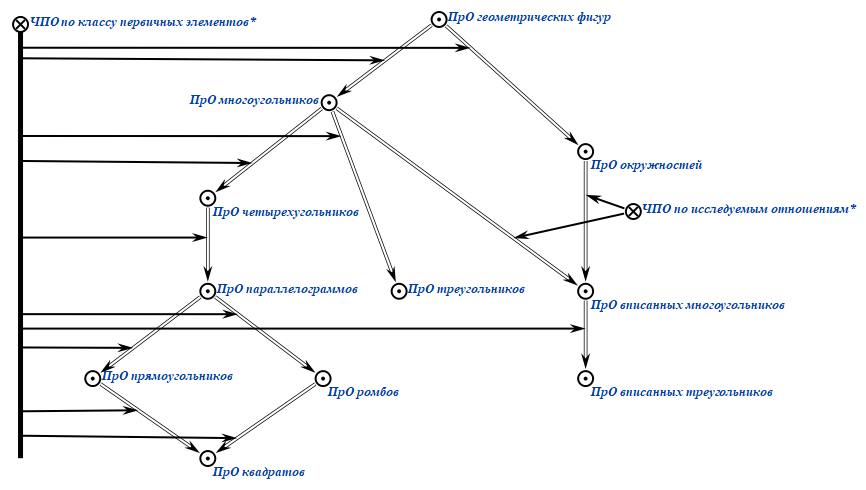
\includegraphics[scale=0.55]{figures/sd_sd/sd_hierarchy.png}
	\end{center}
	
\end{frame}
